\chapter{Power Amplifiers}

\section{Classfication of Power Amplifiers}

Output stages are classified according to the collector current waveform that results when an input signal is applied.

\begin{figure}[H]
  \centering
  \begin{subfigure}{.4\textwidth}
    \centering
    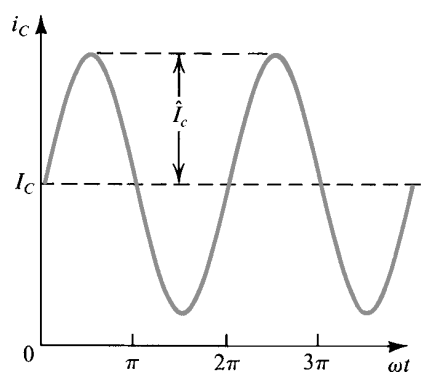
\includegraphics[width=\linewidth]{figures/Power-A}
    \caption{Class A}
  \end{subfigure}
  \begin{subfigure}{.4\textwidth}
    \centering
    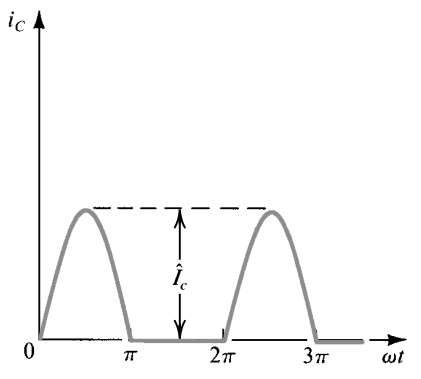
\includegraphics[width=\linewidth]{figures/Power-B}
    \caption{Class B}
  \end{subfigure}
\end{figure}

\begin{figure}[H]
  \centering
  \begin{subfigure}{.4\textwidth}
    \centering
    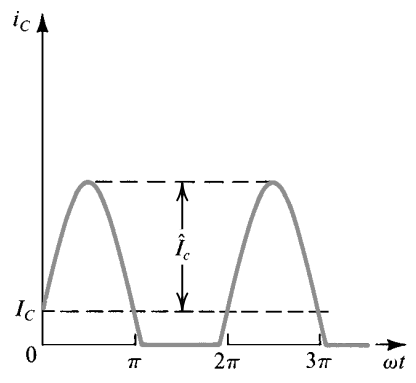
\includegraphics[width=\linewidth]{figures/Power-AB}
    \caption{Class AB}
  \end{subfigure}
  \begin{subfigure}{.4\textwidth}
    \centering
    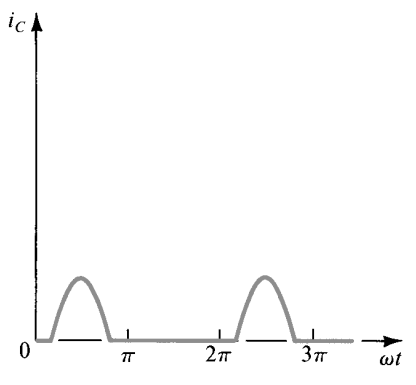
\includegraphics[width=\linewidth]{figures/Power-C}
    \caption{Class C}
  \end{subfigure}
\end{figure}

\section{Some Example Circuits}

\begin{figure}[H]
  \centering
  \begin{subfigure}{.4\textwidth}
    \centering
    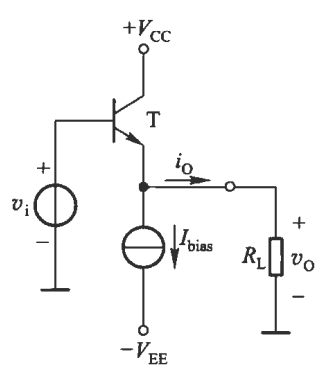
\includegraphics[width=\linewidth]{figures/Power-A-Ex}
    \caption{Class A Output Stage}
  \end{subfigure}
  \begin{subfigure}{.4\textwidth}
    \centering
    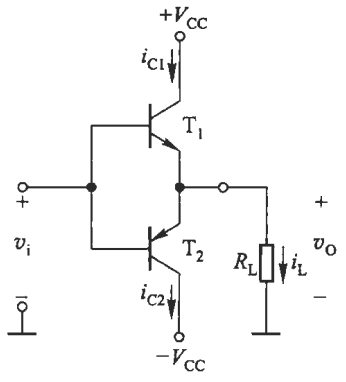
\includegraphics[width=\linewidth]{figures/Power-B-Ex}
    \caption{Class B Output Stage}
  \end{subfigure}
\end{figure}

\section{Power Output}

\begin{equation*}
  \begin{aligned}
    & V_{om} = \dfrac{V_{om+} + V_{om-}}{2} \\
    & P_{om} = \left( \dfrac{V_{om}}{\sqrt{2}}  \right)^2 \cdot \dfrac{1}{R_L}  
  \end{aligned}
\end{equation*}

\section{Crossover Distortion Avoiding}

\begin{figure}[H]
  \centering
  \begin{subfigure}{.45\textwidth}
    \centering
    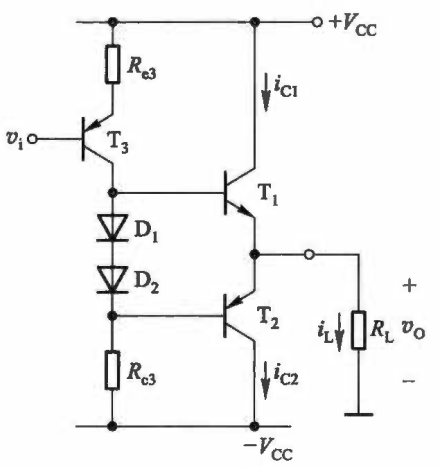
\includegraphics[width=\linewidth]{figures/Power-AB-Ex1}
    \caption{Class AB Output Stage with Double Source}
  \end{subfigure}
  \begin{subfigure}{.45\textwidth}
    \centering
    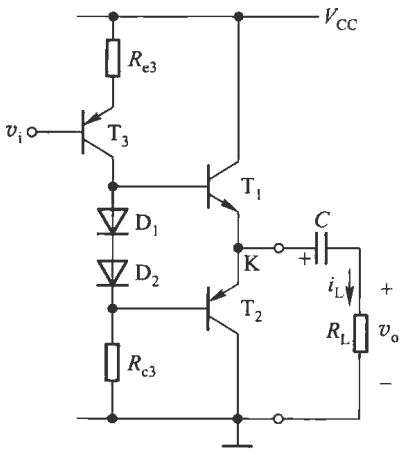
\includegraphics[width=\linewidth]{figures/Power-AB-Ex2}
    \caption{Class AB Output Stage with Single Source}
  \end{subfigure}
\end{figure}

%%% Local Variables:
%%% mode: latex
%%% TeX-master: "Analogue_Electronics"
%%% End:
